\documentclass[a4paper]{scrreprt}

\usepackage[german]{babel}
\usepackage[utf8]{inputenc}
\usepackage[T1]{fontenc}
\usepackage{ae}
\usepackage{amssymb}
\usepackage{graphicx}
\usepackage{hyperref}

\begin{document}

\title{BS Zusammenfassung}
\author{Benedict Hauck, Fedor Scholz\\Alex Tu, Florian Pohl}
\maketitle

\tableofcontents
\vspace{1cm}

\chapter{01aIntro}

\section{Was ist ein Betriebssystem?}
\begin{itemize}
	\item Vermittler zwischen Benutzer und Computer
	\item Ziele
		\begin{itemize}
			\item Benutzerprogramme ausfuehren und dem Benutzer das Loesen von Problemen erleichtern
			\item Computer benutzbarer machen
			\item Hardware des Computer effizient nutzen
			\item Benutzerziele
				\begin{itemize}
					\item Benutzbarkeit
					\item Einfach zu lernen
					\item Zuverlassigkeit
					\item Sicherheit
					\item Schnelligkeit
				\end{itemize}
			\item Systemziele
				\begin{itemize}
					\item Leicht zu designen, implementieren und unterhalten
					\item Flexibilitaet
					\item Zuverlaessigkeit
					\item Fehlerfreiheit
					\item Effizienz
				\end{itemize}
		\end{itemize}
	\item Vier Komponenten eines Computersystems in richtiger Reihenfolge
		\begin{itemize}
			\item Benutzer
			\item System- und Anwendungsprogramme
			\item Betriebssystem
			\item Hardware
		\end{itemize}
	\item Betriebssysteme verteilen Ressourcen
		\begin{itemize}
			\item Verwaltung aller Ressourcen
			\item Entscheidung bei konfligierenden Anfragen fuer effizientes und faires Benutzen der Ressourcen
		\end{itemize}
	\item Betriebssysteme kontrollieren
		\begin{itemize}
			\item Kontrolle der Ausfuehrung von Programmen, um Fehler und Missbrauch des Computers zu verhindern
		\end{itemize}
	\item Immer laufendes Programm ist Kernel, Rest ist System- oder Anwendungsprogramm
	\item Bootstrap program wird beim Starten/Neustarten geladen
		\begin{itemize}
			\item In ROM, EPROM oder FLASH als firmware gespeichert
			\item Initialisiert alle Aspekte des Systems, insbesondere die HW-Komponenten
			\item Laedt den Kernel und startet die Ausfuehrung
		\end{itemize}
\end{itemize}

\section{Organisation}
\begin{itemize}
	\item CPUs und device controllers sind fuer Zugriff auf shared memory ueber Bus verbunden
	\item I/O-Geraete und CPU koennen gleichzeitig ausfuehren
	\item Jeder device controller ist zustaendig fuer einen Geraetetypen
	\item Jeder device controller hat einen lokalen Puffer
	\item CPU bewegt Daten vom/zum Hauptspeicher zu/von lokalen Puffern
	\item I/O ist vom Geraet zum lokalen Puffer des controllers
	\item device controller informiert CPU per interrupts, wenn er fertig ist
\end{itemize}


\section{Interrupts}
\subsection{Haeufige Funktionen von Interrupts}
\begin{itemize}
	\item interrupt gibt Kontrolle an interrupt service routine ueber einen interrupt vector, welcher die Adressen von allen service routines beinhaltet
	\item interrupt architecture muss Adresse der unterbrochenen Intruktion speichern
	\item Einkommende interrupts sind aus, wenn gerade ein anderer bearbeitet wird, um lost interrupts zu verhindern
	\item trap ist ein interrupt, welcher von Software verursacht wurde (wegen eines Fehler oder durch eine Nutzer)
	\item Betriebssysteme sind interrupt driven
\end{itemize}

\subsection{Time interrupts}
\begin{itemize}
	\item Time interrupts um endlose Schleifen und Prozesse zu verhindern
	\item Wird nach bestimmter Zeitspanne ausgefuehrt
	\item Wird vor dem schedulen des Programm aufgesetzt
	\item Eingebettete Systeme haben Watchdog, welcher bis 0 zaehlt und dann resettet
\end{itemize}

\subsection{Interrupt Handling}
\begin{itemize}
	\item Betriebssystem merkt sich Status der CPU, indem es Register und Programmzaehler speichert
	\item Legt Typ des interrupts fest
		\begin{itemize}
			\item polling
			\item vectored interrupt system
		\end{itemize}
\end{itemize}

\section{I/O Struktur}
\subsection{Synchrone oder blockende I/O}
\begin{itemize}
	\item Nachdem I/O beginnt, geht die Kontrolle erst nach Fertigstellung der I/O wieder zum Benutzerprogramm
	\item Wait instruction laesst die CPU idlen
	\item Meistens nur ein I/O Request gleichzeitig
	\item Polling
	\item Signal
	\item Callback function
\end{itemize}

\subsection{Direct Memory Access Structure}
\begin{itemize}
	\item Fuer high-speed I/O, damit diese mit fast der Geschwindigkeit des Hauptspeichers Informationen uebertragen koennen
	\item Device Controller uebertraegt Daten in Bloecken vom Puffer direkt in den Hauptspeicher ohne CPU Eingriff
	\item Nur ein interrupt pro Block
\end{itemize}

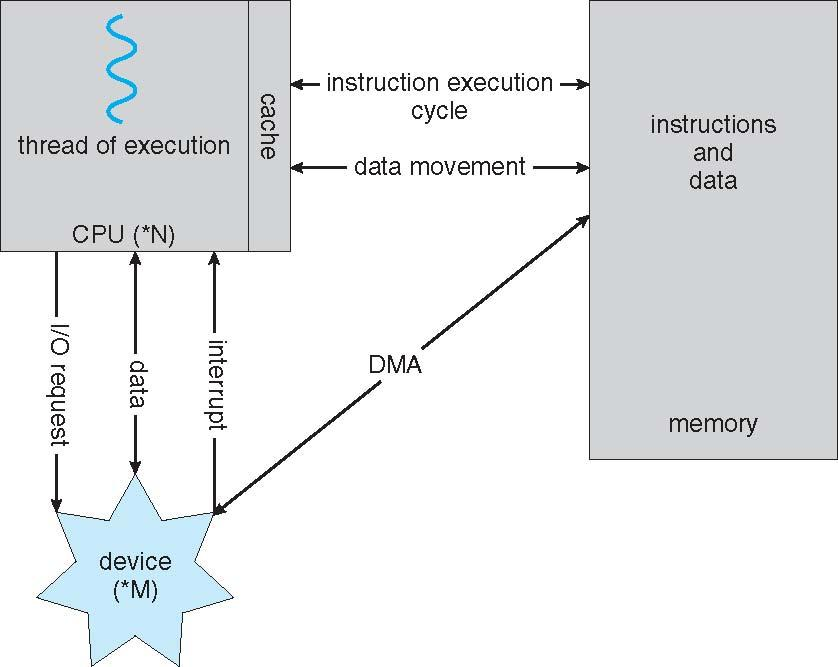
\includegraphics[scale=0.4]{dma.png}

\section{Computer-System Architektur}
\subsection{Multiprozessor-Systeme}
\begin{itemize}
	\item Auch parallel systems, tightly-coupled systems
	\item Vorteile
		\begin{itemize}
			\item Erhoehter Durchsatz
			\item Wirtschaftlichkeit durch große Serie
			\item Erhoehte Zuverlaessigkeit - Fehlertoleranz
		\end{itemize}
	\item Zwei Typen
		\begin{itemize}
			\item Asymmetrische Mehrfachprozessorarchitektur
			\item Symmetrische Mehrfachprozessorarchitektur
		\end{itemize}
	\item Typen von Multiprozessoren
		\begin{itemize}
			\item Multi-socket systems
			\item Multi-Chip Module (MCM) (=Multi-Core)
			\item Chip Multiprocessor (CMP) (=Multi-Core)
			\item Simultaneous MultiThreading Processor (SMT)
		\end{itemize}
\end{itemize}

\subsection{Geclusterte Systeme}
Wie Multiprozessorsystem, nur dass mehrere Systeme zusammen arbeiten

\begin{itemize}
	\item Teilen sich meistens Speicher ueber storage-area network (SAN)
	\item Ermoeglicht hochverfuegbare Services, welche Fehler ueberleben
		\begin{itemize}
			\item Asymmetrisches Clustern hat eine Maschine im hot-standby mode
			\item Symmetrisches Clustern hat viele Maschinen mit laufenden Programmen, welche sich gegenseitig beobachten
			\item Manche sind fuer hochperfomantes computing (HPC)
		\end{itemize}
\end{itemize}

\section{Betriebssystem Struktur}
\begin{itemize}
	\item Multiprogramming ist noetig fuer Effizienz
		\begin{itemize}
			\item Einzelner Benutzer kann nicht CPU und I/O die ganze Zeit auslasten
			\item Multiprogramming organisiert jobs, sodass CPU immer beschaeftigt ist
			\item Untermenge aller Jobs ist im Hauptspeicher
			\item Einer wird ausgewaehlt per job scheduling
			\item Wenn dieser warten muss, wechselt OS den job
		\end{itemize}
	\item Timesharing (multitasking) laesst CPU so schnell jobs wechseln, sodass interaktives computing moeglich ist
		\begin{itemize}
			\item Response time < 1 Sekunde
			\item Jeder Benutzer hat mindestens 1 Programm im Speicher, welches ausgefuehrt wird $\Rightarrow$ process
			\item Wenn mehrere jobs bereit sind $\Rightarrow$ CPU scheduling
			\item Wenn Prozess nicht in Speicher passt $\Rightarrow$ swapping
			\item Virtueller Speicher erlaubt Ausfuehrung von Prozessen nicht komplett im Speicher
		\end{itemize}
\end{itemize}

\section{Uebergang vom User zum Kernel Mode}
\begin{itemize}
	\item Interrupt gesteuert durch Hardware
	\item Softwarefehler oder Anfrage erzeugt exception oder trap
	\item Dual-mode erlaubt es OS, sich und andere Komponenten zu schuetzen
	\item Mode bit bereitgestellt durch HW
		\begin{itemize}
			\item Zeigt an, ob System im User oder Kernel Mode ist
			\item Manche previligierten Instruktionen sind nur im Kernel Mode moeglich
			\item System call aendert Modus zu Kernel, Wiederkehr vom call aender Modus zu User
		\end{itemize}
\end{itemize}

\section{Prozessverwaltung}
\begin{itemize}
	\item Prozess ist ein Programm waehrend der Ausfuehrung: Programm ist eine passive, Prozess eine aktive Einheit
	\item Prozessbeedigung erfordert das freigeben von genutzten Ressourcen
	\item Single-threaded process hat einen program counter und wird sequentiell ausgefuehrt
	\item Multi-threaded process hat einen program counter pro thread
	\item Das Betriebssystem ist dabei fuer folgendes zustaendig:
		\begin{itemize}
			\item Erschaffen und loeschen von Benutzer- und Systemprozessen
			\item Suspenden und resumen von Prozessen
			\item Bereitstellung von Mechanismen fuer Prozessynchronisation
			\item Bereitstellung von Mechanismen fuer Prozeskommunikation
			\item Bereitstellung von Mechanismen fuer das Behandeln von deadlocks
		\end{itemize}
\end{itemize}

\section{Speicher}
\subsection{Storage Structure}
\begin{itemize}
	\item Hauptspeicher - großer Speicher, auf welchen CPU direkt zugreifen kann
	\item Zweitspeicher - Erweiterung des Hauptspeichers, welche groß und nicht fluechtig ist
	\item Magnetische Disks - Oberflaeche in tracks geteilt, welche wiederum aus Sektoren bestehen
\end{itemize}

\subsection{Speicherverwaltung}
\begin{itemize}
	\item Alle Daten muessen vor und nach Verarbeitung im Speicher sein
	\item Alle Instruktionen muessen in der Reihenfolge ihrer Ausfuehrung im Speicher sein
	\item Aktivitaeten des OS
		\begin{itemize}
			\item Darauf achten, wer was im Speicher benutzt
			\item Bestimmen, welche Prozesse und Daten in und aus dem Speicher gehen
			\item Zuteilen und freigeben von Speicherplatz
			\item Einheitlichen, logischen Ueberblick bieten
				\begin{itemize}
					\item Abstrahiert physikalischen Eigenschaften zu logischen Einheiten: Dateien
					\item Jedes Medium wird von einem device kontrolliert
				\end{itemize}
		\end{itemize}
	\item Dateisystemverwaltung
		\begin{itemize}
			\item Dateien haeufig in Ordner organisiert
			\item Kontrolle ueber Zugriff
			\item Aktivitaeten des OS
				\begin{itemize}
					\item Erstellen und Loeschen von Dateien und Ordnern
					\item Grundsaetzliche Moeglichkeiten zum manipulieren von Dateien und Ordnern
					\item Abbilden von Dateien in sekundaere Speicher
					\item Sichern von Dateien auf nichtfluechtige Speicher
				\end{itemize}
		\end{itemize}
\end{itemize}

\subsection{Speicherhierarchie}
Die Speicherhierarchie haengt von folgenden Punkten ab:
\begin{itemize}
	\item Geschwindigkeit
	\item Kosten
	\item Fluechtigkeit
\end{itemize}

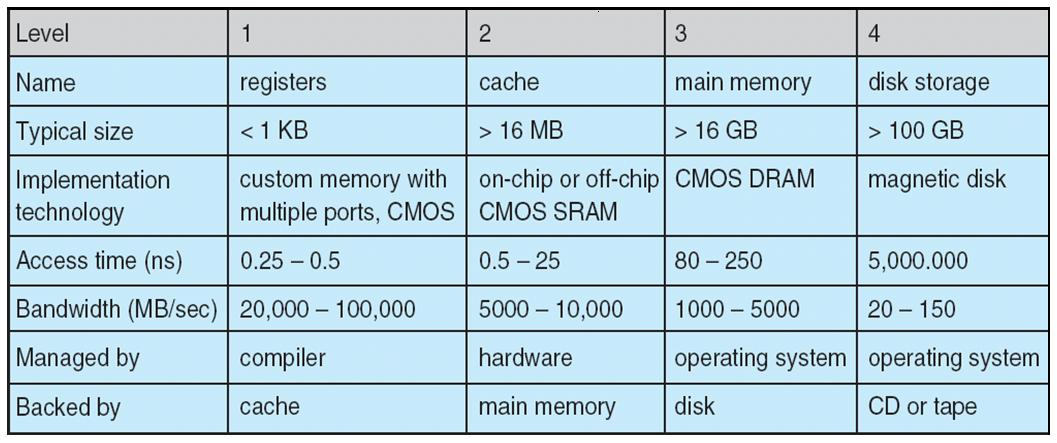
\includegraphics[scale=0.4]{storage.png}

\subsection{Caching}
\begin{itemize}
	\item Wichtiges Prinzip, taucht immer wieder auf (HW, OS, SW)
	\item Benutzte Information wird temporaer von langsameren zu schnelleren Speichern bewegt
	\item Zuerst wird im schnellen Speicher nach Information gesucht
		\begin{itemize}
			\item Wird sie gefunden, wird sie direkt benutzt
			\item Ansonsten wird sie in Cache kopiert und dort benutzt
		\end{itemize}
	\item Cache ist kleiner als Speicher, welcher gecached wird
\end{itemize}

\section{I/O Subsystem}
\begin{itemize}
	\item Betriebssysteme verstehen Eigenheiten der HW vor dem Nutzer
	\item I/O Subsystem ist verantwortlich fuer
		\begin{itemize}
			\item Speicherverwaltung der I/O inklusive Puffern, Cachen, Spoolen
			\item generelles Geraetetreiber-Schnittstelle
			\item Treiber fuer bestimmte Hardwaregeraete
		\end{itemize}
\end{itemize}

\section{Schutz und Sicherheit}
\begin{itemize}
	\item Schutz - Jeder Mechanismus, welches den Zugriff von Prozessen und Nutzern auf Ressourcen kontrolliert
	\item Sicherheit - Verteildigung des System gegen interne und externe Attacken
	\item Systeme unterscheiden meistens zunaechst nach Nutzer
		\begin{itemize}
			\item Nutzeridentitaeten (user IDs) behinhalten Namen und Nummer
			\item User ID ist mit alles Dateien und Prozessen verknuepft, auf die der Nutzer zugreifen darf
			\item Gruppenidentitaeten (group IDs) erlauben den Zugriff einer Menge von Benutzern
			\item Privilege escalation erlaubt es Nutzern, die ID zu wechseln
		\end{itemize}
\end{itemize}

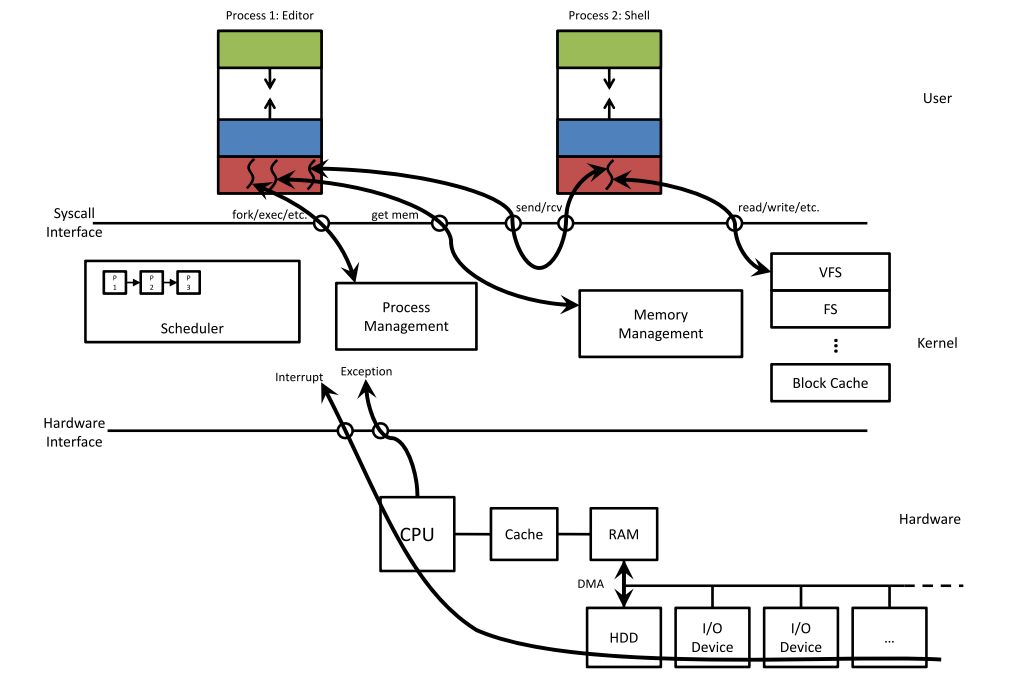
\includegraphics[scale=0.5]{big_picture.png}

\section{Design und Implementierung von OS}
\begin{itemize}
	\item Policy: Was wird getan?
	\item Mechanism: Wie wird es getan?
\end{itemize}

\section{OS Service}
\begin{itemize}
	\item Benutzerschnittstelle (CLI, GUI, Batch)
	\item Programmausfuehrung
	\item I/O Operationen
	\item Dateisystemmanipulationen
	\item Kommunikationen: Prozesse tauschen Informationen aus (shared memory oder message passing)
	\item Fehlererkennung
		\begin{itemize}
			\item Findet in CPU, Speicher, I/O Geraeten und Benutzerprogrammen statt
			\item Fuer jeden Typ von Fehler, hat das OS definierte Aktionen
			\item Debugmoeglichkeiten erhoehen Effizienz des Nutzen
		\end{itemize}
	\item Ressourcenallokation: s.o.
	\item Accouting: Welcher Nutzer nutzt wieviel?
	\item Schutz und Sicherheit: Besitzer von Informationen wollen Kontrolle ueber ihre Benutzung, Prozesse sollen nicht interferieren
		\begin{itemize}
			\item Schutz: Jeder Zugriff auf das System wird kontrolliert
			\item Sicherheit: Authentifikation
		\end{itemize}
\end{itemize}

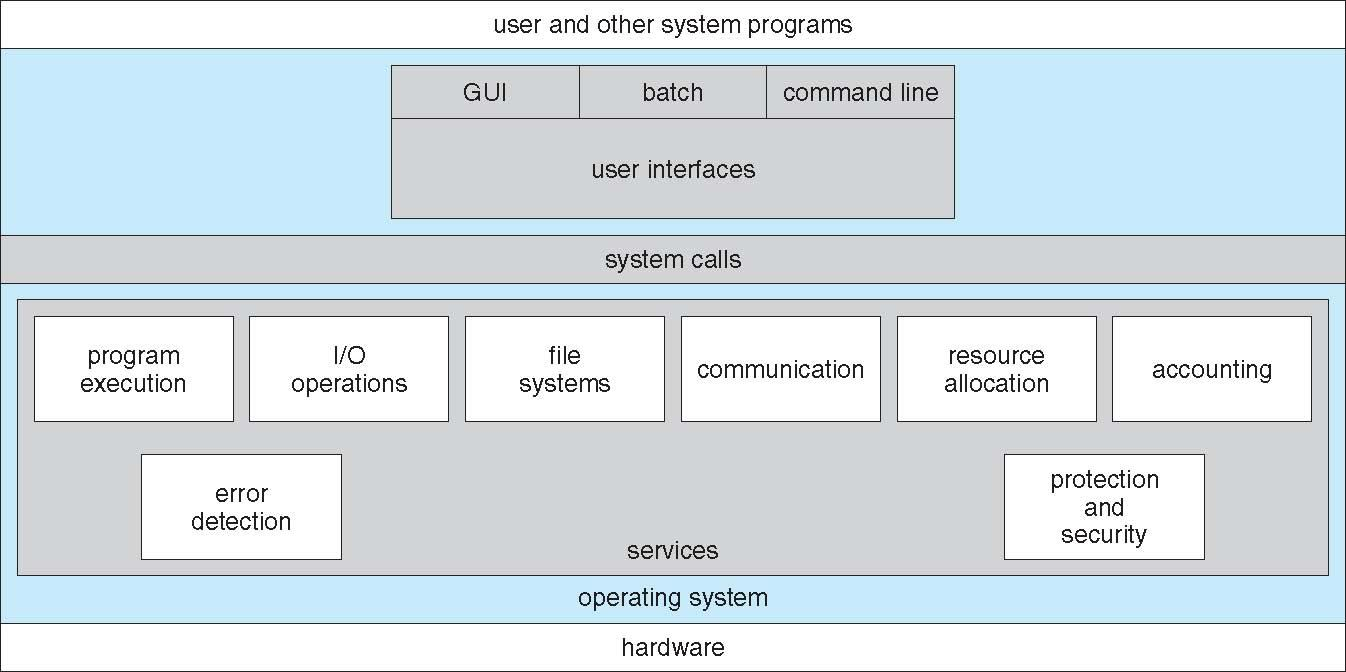
\includegraphics[scale=0.35]{services.png}

\subsection{System Calls}
\begin{itemize}
	\item Schnittstelle zu den Services vom OS
	\item Meisten in hoeher Sprache geschrieben
	\item Meistens ueber ein Application Program Interface (API) genutzt
	\item Win32 API, POSIX API, Java API
\end{itemize}

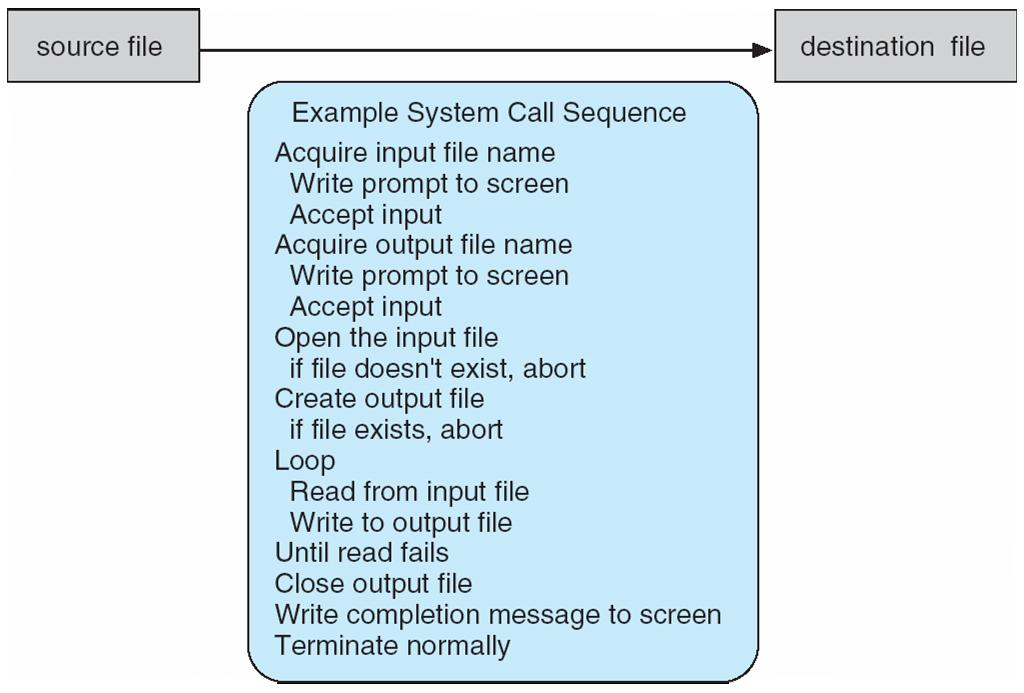
\includegraphics[scale=0.3]{system_call.png}

\subsubsection{Beispiel fuer API}

ReadFile() Funktion in der Win32 API zum Lesen einer Datei:\\

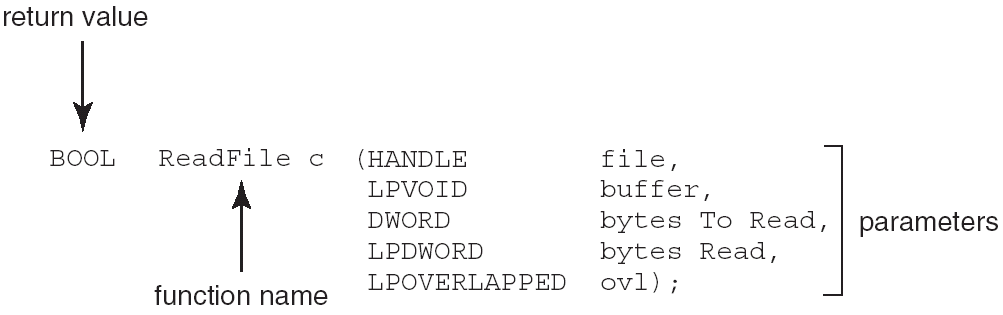
\includegraphics[scale=0.4]{api.png}

\begin{itemize}
	\item HAND: Zu lesende Datei
	\item LPVOID: Puffer, in den die Datei gelesen wird
	\item DWORD: Anzahl der zu lesenden Bytes
	\item LPDWORD: Anzahl der bereits gelesen Bytes
	\item LPOVERLAPPED: Gibt an, ob ueberlappende I/O genutzt wird
\end{itemize}

\subsubsection{Implementierung der System Calls}
\begin{itemize}
	\item Fuer jeden System Call gibt es eine Nummer
	\item System Call Schnittstelle veranlasst einen System Call im OS Kernel und gibt den Status sowie die Rueckgabewerte zurueck
	\item Aufrufer braucht nichts ueber die Implementierung zu wissen
\end{itemize}

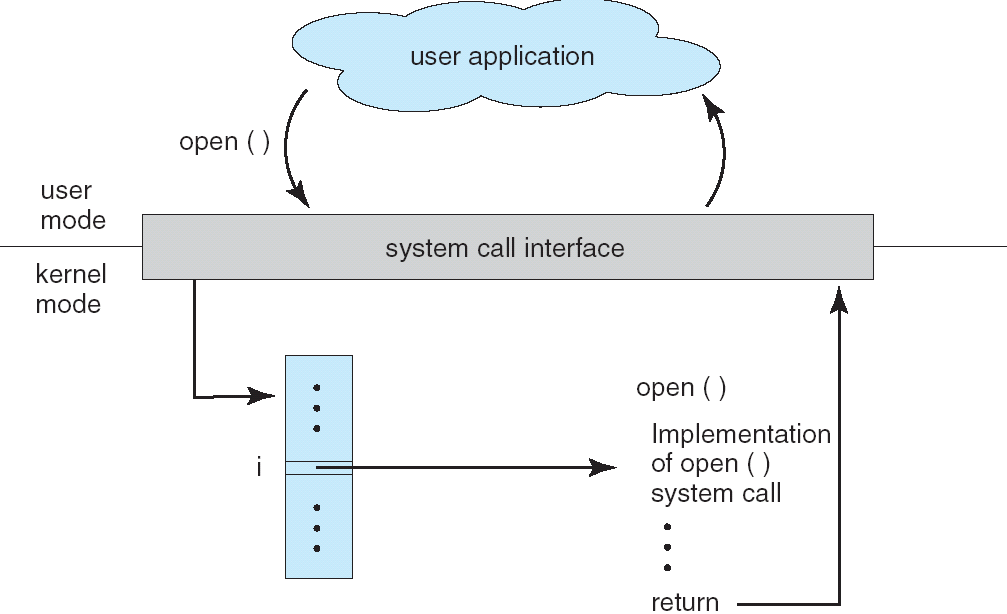
\includegraphics[scale=0.4]{syscall_os_relationship.png}

\subsubsection{Beispiel fuer C Bibliothek}

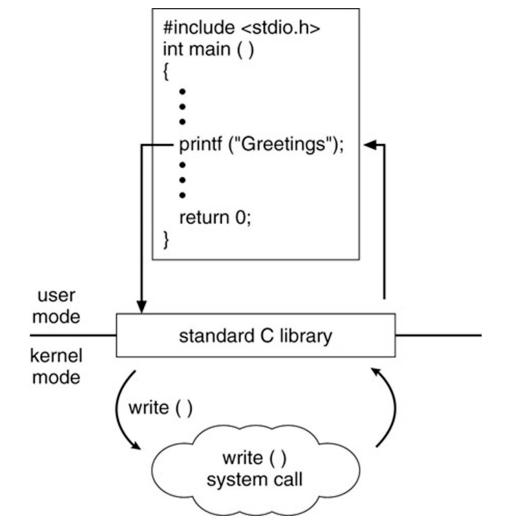
\includegraphics[scale=0.4]{printf.png}

\subsubsection{Parameter}
Generell gibt es drei Methoden, Parameter an das OS zu uebergeben:
\begin{itemize}
	\item Durch Register, manchmal gibt es aber mehr Parameter als Register
	\item Durch einen Block, wobei seine Adresse ueber Register uebergeben wird
	\item Durch Pushen auf den Stack
\end{itemize}

\subsubsection{System Calls von Windows und Unix}
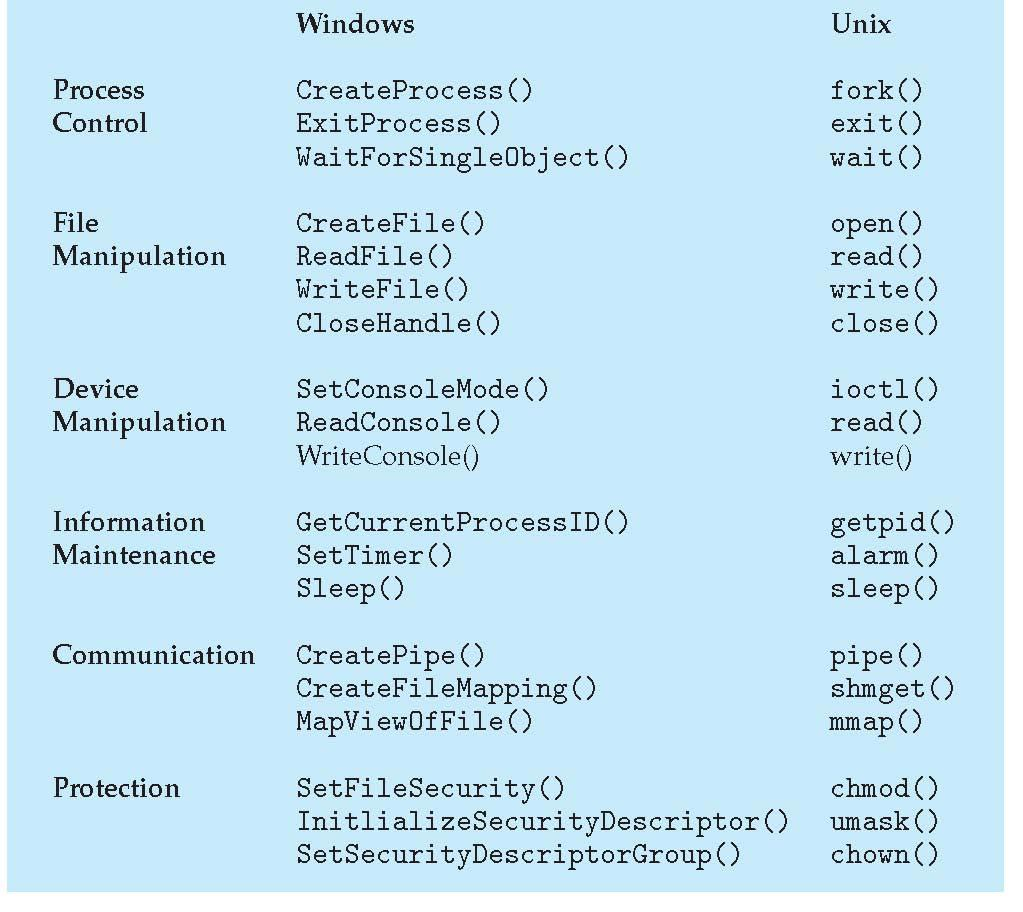
\includegraphics[scale=0.3]{syscall_examples.png}

\subsection{System Programs}
Systemprogramme ermoeglichen angenehme Umgebung fuer Programmentwicklung und -ausfuehrung:
\begin{itemize}
	\item Dateimanipulation
	\item Statusinformationen
	\item Dateimodifikation
	\item Support fuer Programmiersprachen
	\item Laden und Ausfuehren von Programmen
	\item Kommunikation
	\item Applikationen
\end{itemize}
Meisten geht die Sicht des Benutzer ueber Systemprogramme anstatt ueber Systemcalls.












\chapter{01bCProgramming}
\chapter{02OS}

\section{Monolithisches System}
Vorteile:
	\begin{itemize} 
		\item Einfacher Zugriff auf alle Systemdaten 
		\item Kosten von Modulinteraktionen sind niedrig
		\item Erweiterbar über Schnittstellen
		\item Vorhersehbares Verhalten 
	\end{itemize}
Nachteile:
	\begin{itemize}
		\item Kein Schutz zwischen System und Anwendung
		\item Instabil
	\end{itemize}

Beispiele:
	\begin{itemize}
		\item uCLinux, RTOSe, eCos
	\end{itemize}
	
\section{Mehrschichtiger Ansatz}
	\begin{itemize}
		\item Betriebssystem ist in n Schichten aufgeteilt
		\item Jede Schicht kann nur auf die Funktionen und Dienste von niedrigeren Schichten zugreifen 
			\begin{itemize} 
				\item Schicht 0 ist die Hardware
				\item Schicht n ist das Benutzerinterface
			\end{itemize}
		\item Einfachere Migration zwischen Plattformen
		\item Einfachere Evolution der Hardwareplattform
		\item Niedrigere Schichten implementieren Mechanismen
		\item Höhere Schichten implementieren meistens Policies
	\end{itemize}

\begin{center}
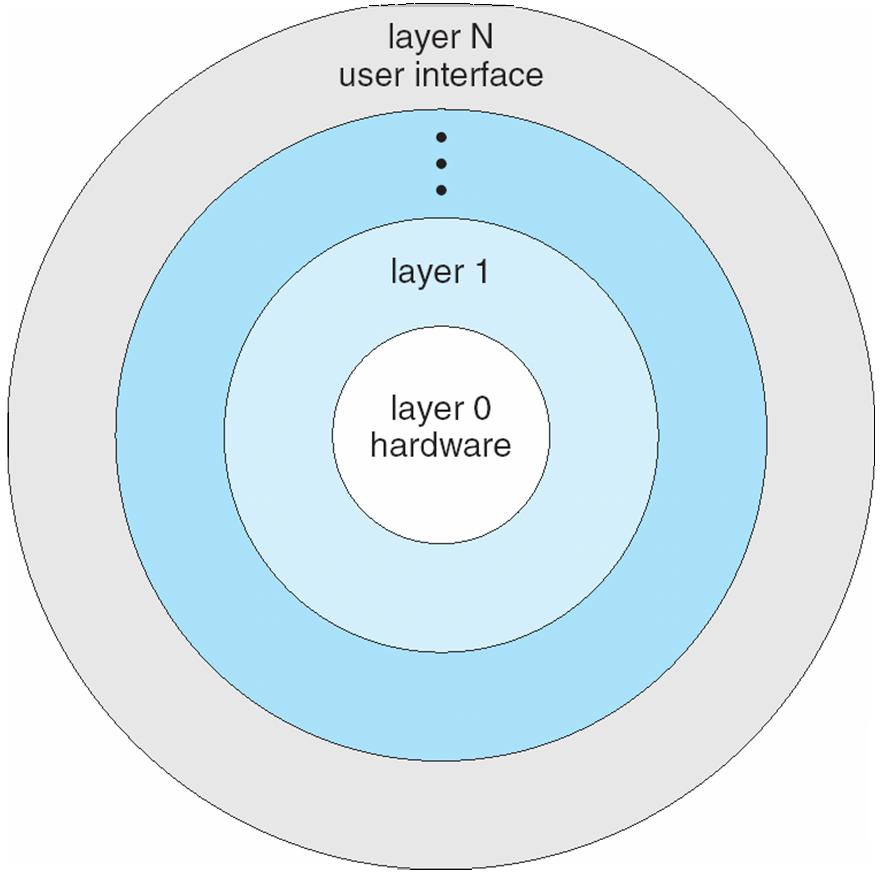
\includegraphics[scale=0.15] {schichtenmodell.png} 
\end{center}

Vorteile:
	\begin{itemize}
		\item Jede Schicht kann unabhängig getestet und verfiziert werden
		\item Korrektheit von Schicht n hängt nur von Schicht n-1 ab (einfacheres Debugging, einfachere Wartung)
	\end{itemize}

Nachteile:
	\begin{itemize}
		\item Nur unidirektionaler Schutz
		\item Beiseitige Abhängigkeit von Schichten verhindert strikte Schichtenbildung
	\end{itemize}
Beispiele:
	\begin{itemize}
		\item THE (Dijkstra), Multics(GE), VOCOS(EWSD)
	\end{itemize}
	
\section{Monolitische Kernels}
	\begin{center}
		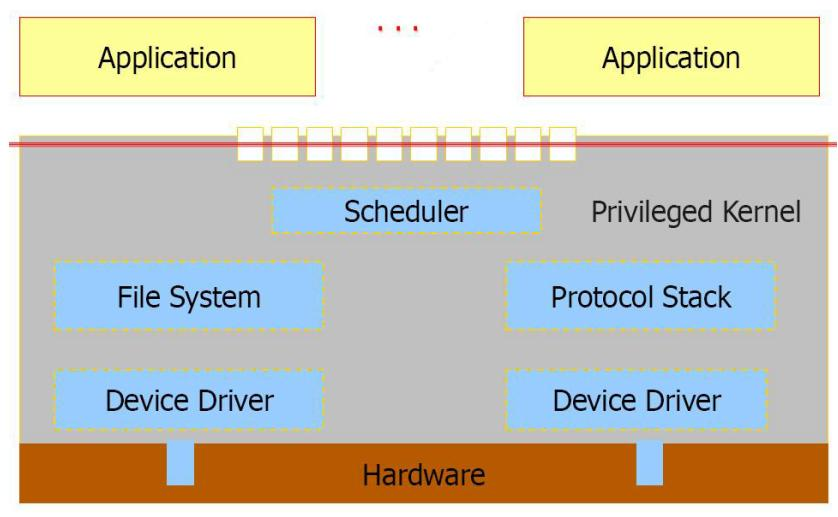
\includegraphics[scale=0.3] {monolithickernel.png}
	\end{center}
	Vorteile:
		\begin{itemize}
			\item "Gute" Performance
			\item Ausreichender Schutz zwischen Anwendungen
			\item Erweiterbar über Schnittstellen und statische/ladbare Module
		\end{itemize}
	Nachteile:
		\begin{itemize}
			\item Kein Schutz zwischen Kernel-Komponenten
			\item Nebeneffekte durch undokumentierte Interfaces
			\item Hohe Komplexität durch hohe gegenseitige Abhängigkeit
		\end{itemize}
	Beispiele
		\begin{itemize}
			\item Linux, Solaris
		\end{itemize}

\section{Microkernel Systeme}
	\begin{center}
		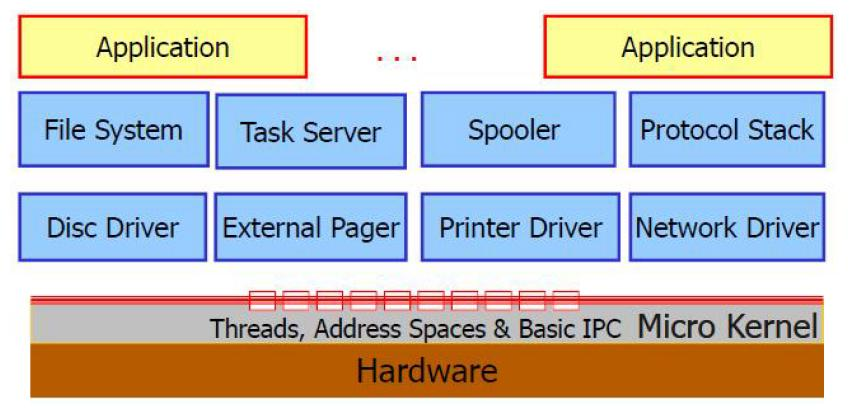
\includegraphics[scale=0.3] {microkernel.png}
	\end{center}

	\begin{itemize}
		\item Möglichst viel des Kernels in den "Benutzer" space packen
		\item Kommunikation erfolgt zwischen Benutzermodulen mit Nachrichtenweitergabe
	\end{itemize}
	
	Vorteile:
		\begin{itemize}
			\item Einfacher einen Microkernel zu erweitern
			\item Einfacher das Betriebssystem auf neue Architekturen zu portieren
			\item Zuverlässiger (es läuft weniger Code im Kernel-Modul
			\item Mehrere APIs vorhanden
			\item Verbesserte Robustheit und Sicherheit
			\item Einfacher zum Testen und Beweisen
			\item Verbesserte Wartbarkeit
		\end{itemize}
	Nachteile:
		\begin{itemize}
			\item Performance Unkosten durch Kommunikation von Benutzerspace zum Kernelspace 
			\item Zusätzliche Zersetzung
			\item Schlechte Erfahrungen mit IBMs Workplace OS (1991-1995)
		\end{itemize}

\section{Virtuelle Maschinen}
	\begin{itemize}
		\item Eine virtuelle Maschine nimmt den mehrschichtigen Ansatz und behandelt Hardware sowie den Kernel des Betriebssystems so als wären sie Hardware
		\item Eine virtuelle Maschine stellt ein identisches Interface zu der blanken, darunterliegenden Hardware
		\item Der Betriebssystem-Host kreiert die Illusion das ein Prozess sein eigenen Prozessor und (virtuellen Speicher) hat.
		\item Jeder Gast bekommt eine Kopie des darunterliegenden Computers zur Verfügung gestellt.
	\end{itemize}
	Vorteile:
		\begin{itemize}
			\item Mehrere Betriebssysteme können sich die gleiche Hardware teilen
			\item Gegenseitiger Schutz
			\item Nützlich für Development und Testen
		\end{itemize}
	\begin{center}
		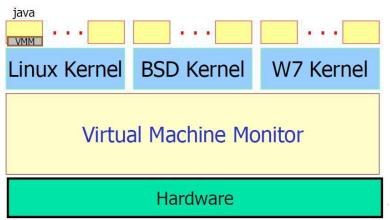
\includegraphics[scale=0.5] {virtualmachine.png}
		\\
		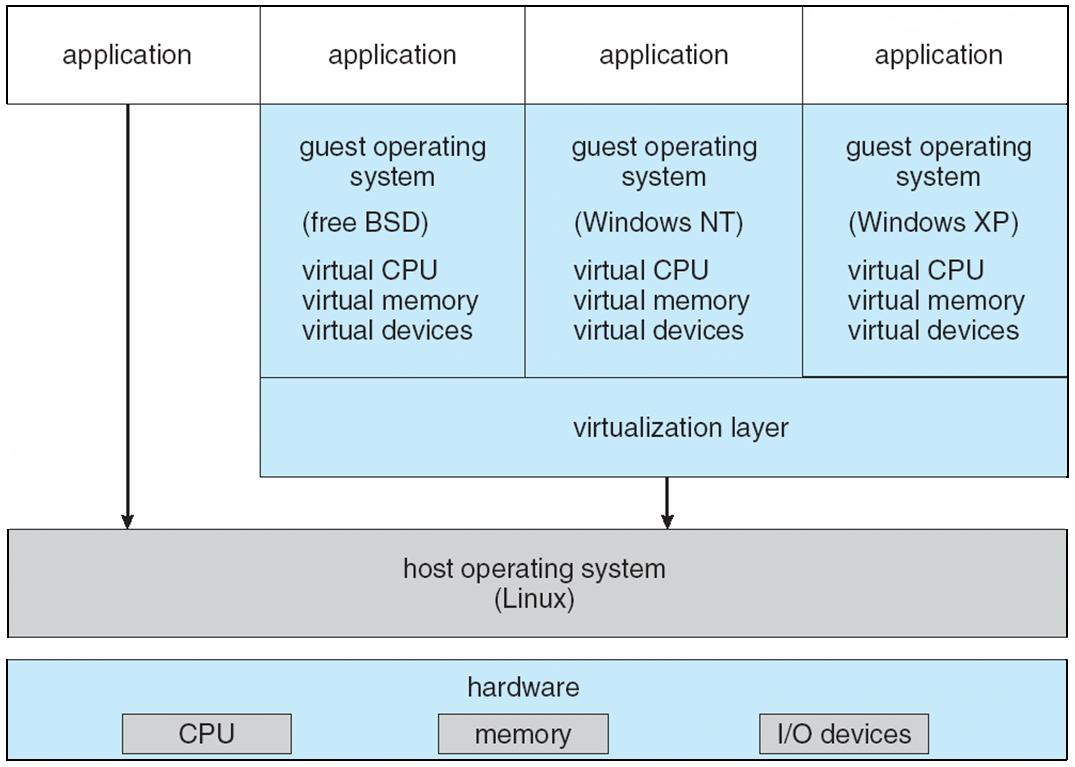
\includegraphics[scale=0.35] {vmwarearchi.png}
		\\
		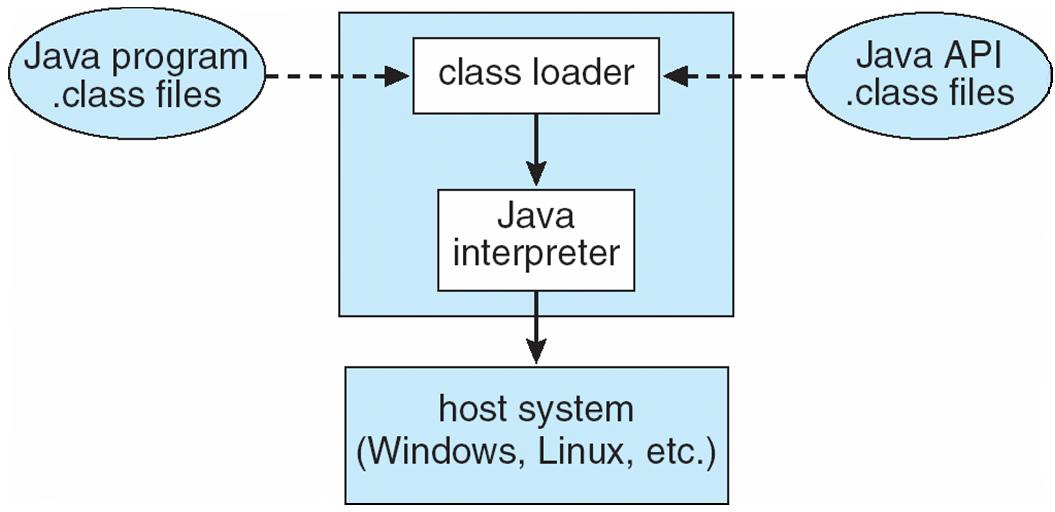
\includegraphics[scale=0.3] {javavm.png}
	\end{center}


\chapter{03aProcess-management}
\chapter{03bProcess-management-scheduling}
\chapter{04Process-coordination}

\section{Interprozess Kommunikation}
	\begin{itemize}
		\item Prozesse in einem System können unabhängig oder zusammenarbeitend sein
		\item Zusammenarbeitende Prozesse können sich andere oder von anderen Prozessen beeinflusst werden
		\item Zusammenarbeitende Prozesse benötigen interprocess communication (IPC -> 2 Modelle: Shared memory, message passing)
	\end{itemize}
	Gründe für zusammenarbeitende Prozesse:
	\begin{itemize}
		\item Schnellere Berechnung
		\item Kompfort/Einfachheit
		\item Modularität
		\item Teilen von Informationen
	\end{itemize}

\subsection{Nachrichtenweitergabe (Message Passing)}
	\begin{itemize}
		\item Mechanismus für Prozesse um zu kommunizieren und ihre Aktionen zu synchronisieren
		\item IPC-Einrichtung bietet zwei Operationen: receive, send (Nachrichtengröße ist fix oder variabel)
	\end{itemize}
\subsubsection {Direkte Kommunikation}
	\begin{itemize}
		\item Prozesse müssen sich gegenseitig explizit per Namen nennen
		\item send(P, Nachricht) - schicke eine Nachricht an Prozess P
	\end{itemize}
	Eigenschaften:
	\begin{itemize}
		\item Links werden automatisch eingerichtet
		\item Ein Link wird genau mit einem Paar von kommunizierenden Prozessen assoziiert
		\item Jedes Paar besitzt genau einen Link
		\item Ein Link könnte unidirektional sein, ist aber meistens bi-direktional
	\end{itemize}
	
\subsubsection{Indirekte Kommunikation}
	\begin{itemize}
		\item Nachrichten werden von Mailboxes (ports) gelenkt und empfangen
		\item Jede Mailbox hat eine einzigartige ID
		\item Prozesse können nur kommunizieren wenn sie eine Mailbox teilen
	\end{itemize}
	Eigenschaften:
	\begin{itemize}
		\item Ein Link wird nur eingerichtet falls Prozssse eine Mailbox teilen
		\item Ein Link kann mit vielen Prozessen assoziiert werden
		\item Jedes Paar von Prozessen kann mehere Kommunikationslinks teilen
		\item Links können unidirektional oder bi-direktional sein
	\end{itemize}
	Operationen:
	\begin{itemize}
		\item Neue Mailbox erstellen
		\item schicken und empfangen von Nachrichten über die Mailbox
		\item Mailbox löschen
	\end{itemize}
	
\section{Synchronisation}
	\subsection {Producer-Consumer Problem}
		\begin{itemize}
			\item Problemstellung der Prozesssynchronisation die eine Regelung der Zugriffsreihenfolge auf einer Datenstruktur von Prozessen bzw Thread thematisiert
			\item Prozesse sind Erzeuger oder Verbraucher
		\end{itemize}	
	\subsubsection{Critical-Section-Problem}
		\begin{itemize}
			\item Mutual Exclusion: Wenn Prozess P in seinem kritischen Bereich ist, kann kein anderer Prozess in seinen kritischen Bereich
			\item Progress:  Wenn kein Prozess in seinem kritischen Bereich ausgeführt wird, aber mehrere Prozesse den kritischen Bereich betreten möchten, kann die Auswahl der Prozesse die als nächstes eintreten nicht unbegrenzt aufgeschoben werden
			\item Bounded Waiting: Es muss eine zeitliche Grenze existieren, sodass Prozesse nicht verhungern. (z.B. Prozess A,B wechseln sich in im kritischen Bereich ab obwohl Prozess C auch den kritischen Bereich betreten möchte, Prozess C verhungert)
			\item Viele Systeme bieten Hardwaresupport für critical section code
		\end{itemize}
	\subsection{Semaphore}
		\begin{itemize}
			\item Synchronisationstool das kein "busy waiting" benötigt
			\item Weniger kompliziert
			\item Nur zwei Standardoperationen für die Modifikation eines Semaphores erlaubt: wait(), signal()
			\item Counting semaphore - integer Wert unbegrenzt
			\item Binary semaphore - integer Wert kann zwischen 0 und 1 variieren 
		\end{itemize}

\section{Deadlock and Starvation}
		\begin{itemize}
			\item Deadlock - zwei oder mehr Prozesse warten unbegrenzt auf eine Aktion die nur von einem wartenden Prozess ausgeführt werden kann
			\item Starvation - Ein Prozess könnte nie von einer Semaphorewarteschlange entfernt werden
			\item Priority Inversion - Scheduling-Problem, wenn ein Prozess niedriger Priorität einen Platz hält den ein Prozess höherer Priorität braucht
		\end{itemize}

\chapter{05aMemoryManagement}
\section{Background}
\begin{itemize}
\item Damit ein Programm laufen kann muss es von der Platte in den Speicher gebracht und innerhalb des Prozesses plaziert werden.

\item Auf Hauptspeicher und Register kann nur die CPU direkt zugreifen.

\item Ein Register Zugriff beträgt einen CPU Takt (oder weniger)

\item Hauptspeicher kann einige Zyklen dauern.

\item Cache liegt zwischen Hauptspeicher und CPU Registern

\item Sicherheit des Speichers werden zur Sicherstellung korrek ausgeführter Operationen benötigt.

\end{itemize}

\subsection{Speicherpartitionierung}

Hauptspeicher wird normalerweise in zwei Partitionen unterteilt :
\begin{description}
\item[Resident operating system]\ \\ werden normalerweise im "`low memory"' mit  \textit{interrupt vector} gespeichert
\item[User processes]\ \\werden im "`high memory"' gespeichert
\end{description}

Register dienten dem Schutz der Benutzerprozesse untereinander und vor Veränderungen von Betriebssystemcode und Daten.
\begin{itemize}
\item "`Base register"' beinhalten den Wert der kleinsten physichen Adresse.
\item "`Limit register"' beinhalten den Umfang der logischen Adressen.
\end{itemize}

\begin{center}
		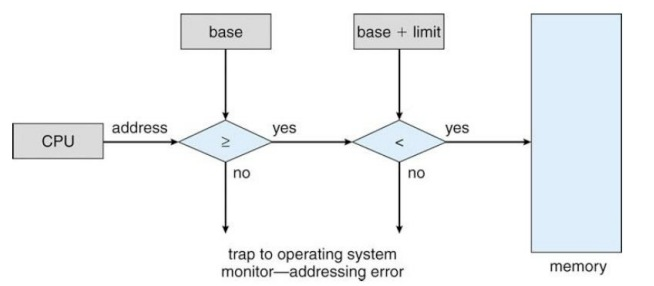
\includegraphics[scale=0.5] {baseandlimit.png}
\end{center}

\subsection{Einfacher Schutz mit \textit{base} und \textit{limit register}}

Ein Paar aus base und limit Registern definieren einen logischen Adressraum

\begin{center}
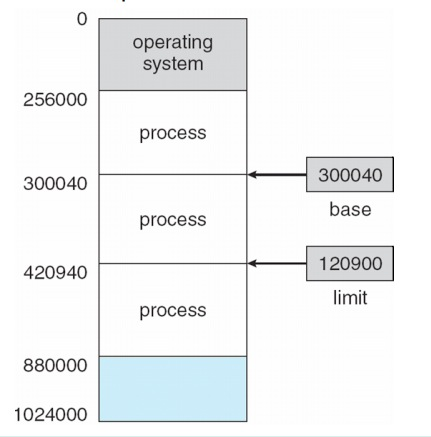
\includegraphics[scale=0.5]{baseandlimitprotection.png}
\end{center}


\section{Swapping}
\begin{itemize}
\item Ein Prozess kann temporär aus dem Speicher in einen Zusatzspeicher gewechselt werden und dann wieder zurück um die Ausführung fortzusetzen
\item \textbf{Zusatzspeicher (\textit{Backing store})} \ \\ Schneller Speicher, welcher groß genug ist um alle \textit{memory images} aller Nutzer unterzubringen. Er muss jedoch direkten Zugriff zu jenen bieten.
\item \textbf{Roll out, roll in} \ \\ Eine Swapping Variation für prioritätsbasierte scheduling Algorithmen: Prozesse niedriger Priorität werden mit Prozessen hoher Priorität ausgewechselt um somit geladen und ausgeführt werden können.
\item Hauptbestandteil der \textit{swap time} ist die \textit{transfer time}: Die totale Transferzeit ist direkt proportional zur Menge des ausgewechelten Speichers
\item Modifizierte Versionen von ˆ\textit{swapping} wird auf vielen System gefunden (z.B UNIX, Linux und Windows)
\item Das System führt eine \textit{ready queue} mit "`ready to run"'-Prozessen welche ein memory image im Speicher haben.

\end{itemize}

\begin{figure}[ht]
\centering
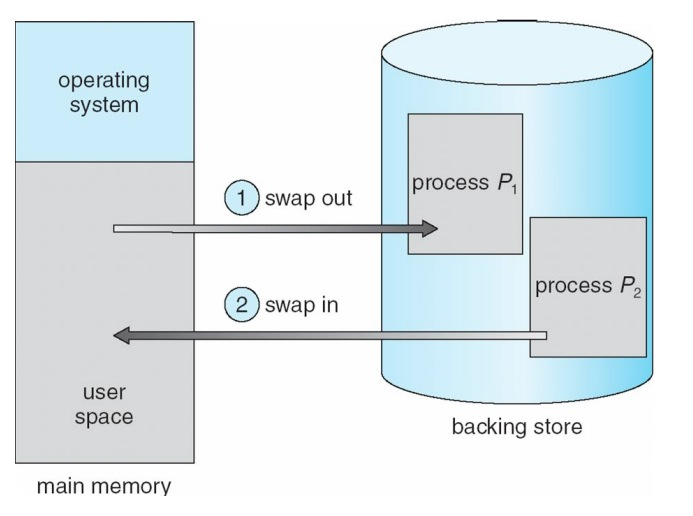
\includegraphics[scale=0.6]{swapping.png}
\caption{Schematik von Swapping}
\end{figure}

\section{Allocation}
\subsection{Zusammenhängende Allokierung (\textit{contiguous allocation)}}
\subsubsection{Multiple Partitions Allokierung}
\begin{itemize}
\item \textit{Hole}: Blöcke an verfügbarem Speicher. Löcher verschiedener Größe sind über den ganzen Speicher verteilt
\item Bei Ankunft eines Prozesses, wird Speicher von einem Loch, welches groß genug ist um den Prozess aufzufassen, allokiert
\end{itemize} Das Betriebssystem kümmert sich um Informationen über:

\begin{itemize}
\item[a)] allokierte Partitionen
\item[b)] freie Partitionen (Löcher)
\end{itemize}

\begin{figure}[ht]
\centering
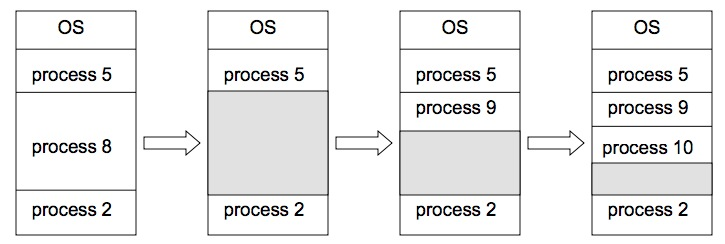
\includegraphics[scale=0.6]{allocation.png}
\caption{Schematik Speicherallokierung}
\end{figure}

\subsection{Dynamisches Speicher-Allokations Problem}
\textbf{Problem:} Wie befreidigt man Anfragen der Größe n von einer Liste mit freien Löchern?
\begin{itemize}
\item \textit{First-fit}: Allokiert das erste Loch, welches groß genug ist: schnellste Allokierungsstrategie, hinterlässt jedoch Löcher unterschiedlicher Größe
\item \textit{Best-fit}: Allokiert das kleinste passende Loch. Es muss jedoch die komplette Liste durchsucht werden, außer sie ist nach Größe sortiert. Hinterlässt die kleinsten Löcher.
\item \textit{Worst-fit}: Allokiert das größte Loch. Es muss die gesammte Liste durchsucht werden, hinterlässt die größten Löcher
\item \textit{Next-fit}: Nächst passendes Loch nach der letzten Allokierung
\item \textit{Buddy System}:
\begin{itemize}
\item Die Löcher werden in k Listen so einsortiert, dass die i-te Liste jeweils Löcher der Länge gleich $2^i/$ für i = 1,...,k enthält
\item Dabei können zwei benachbarte Löcher der i-ten Liste effizient zu einem  Loch der i+1-ten Liste zusammengefügt werden
\item Umgekehrt kann ein Loch der i-ten Liste einfach in zwei Löcher der i-1-ten Listen aufgeteilt werden
\item Löcher im Buddy-System können effizient mittels eines Binärbaumes dargestellt werden
\item Laufzeitverhalten: Zuweisen und Freigabe Block schneller als first/best-fit. Fragmentierungsbehandlung ist aufwändiger. Deshalb Lazy-\textbf{Buddy:Zusammenfügen "`selten"'}
\item Standard für Unix/Linux
\end{itemize}
\end{itemize}

\begin{figure}[ht]
\centering
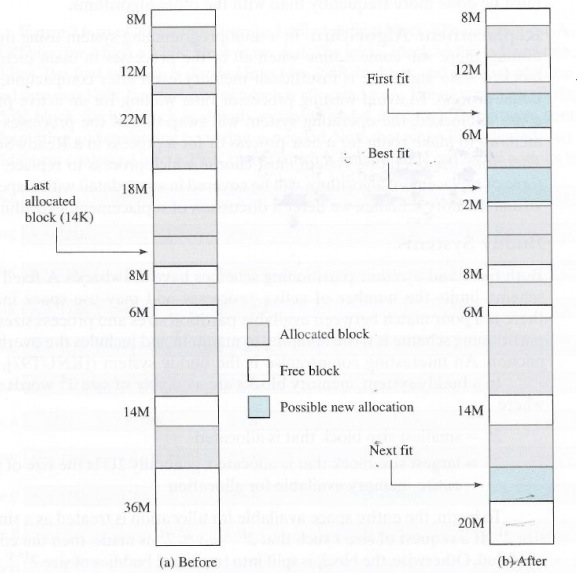
\includegraphics[scale=0.55]{allocationexample.png}
\caption{Beispiel vor und nach Allokierung eines 16Mbyte Blocks}
\end{figure}

\begin{figure}[ht]
\centering
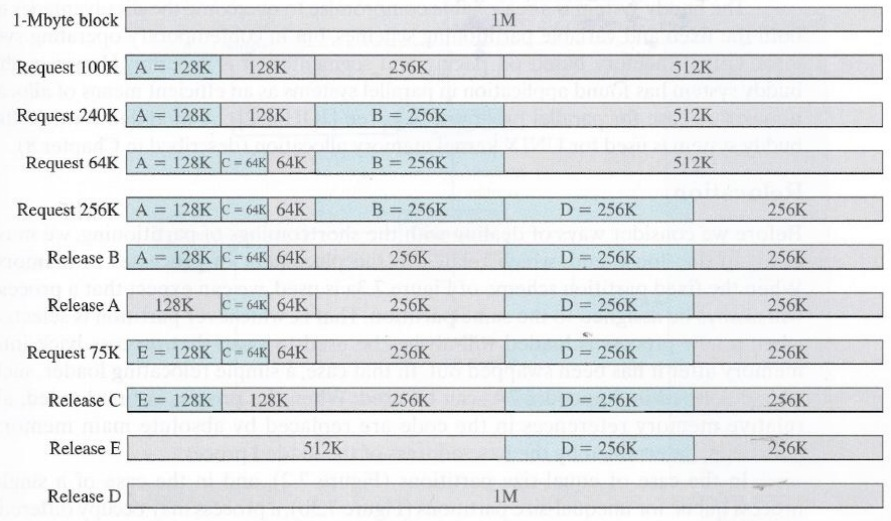
\includegraphics[scale=0.50]{buddysystem.png}
\caption{Beispiel Buddysystem}
\end{figure}
  \ \\
\begin{figure}[ht]
\centering
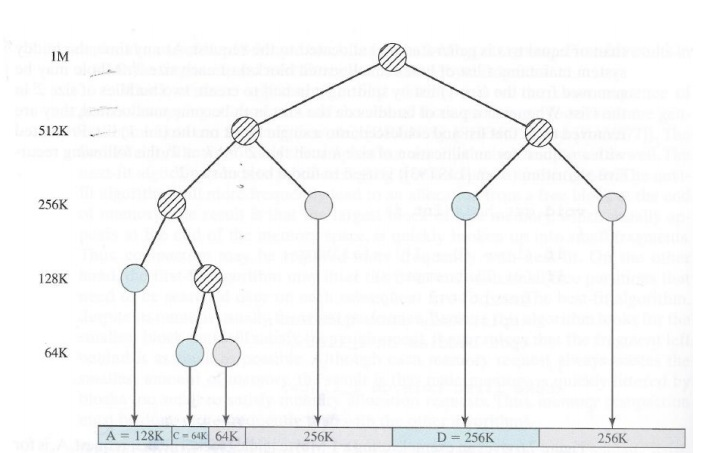
\includegraphics[scale=0.5]{buddysystemtree.png}
\caption{Darstellung Buddysystem als Baum}
\end{figure}
\newpage

\section{Relocation}
\subsection{Fragmentierung}
\begin{itemize}
\item \textbf{Externe Fragmentierung} - Es ist genügend Speicher vorhanden um eine Anfrage zu befriedigen, jedoch nicht zusammenhängend.
\item \textbf{Interne Fragmentierung} - Allokierter Speicher kann ein wenige größer als der angeforderte Speicher sein: Der Größenunterschied ist Speicherintern innerhalb einer Partition, wird jedoch nicht verwendet
\item Reduzierung externer Fragmentierung durch Verdichtung (\textit{compatction}):
\begin{itemize}
\item Vermische den Speicherinhalt um alle freien Speicher in einem großen Block zu sammeln
\item \textit{Compaction} ist nur dann möglich wenn die \textit{relocation} dynamisch und während der Durchführungszeit statt findet

\end{itemize}
\end{itemize}
\subsection{Addressbinding und "`Data to Memory"'}

\begin{itemize}
\item \textbf{Compile time}: Wenn der Speicherstelle  a priori bekannt ist, kann ein absoluter Code generiert werden. Muss jedoch recompiliert werden wenn der Startpunkt verändert wir.
\item \textbf{Load time}: Muss versetzbaren (engl.: \textit{relocatable}) Code generieren wenn die Speicherstelle zur Übersetzungszeit nicht bekannt ist.
\item \textbf{Execution time}: \begin{LARGE}
\textbf{lol wut kein plan, 5a, Folie 17}
\end{LARGE}
\end{itemize}

\subsection{Logische vs. Physicher Adressraum}

\begin{itemize}
\item \textbf{logische Adresse} - CPU generiert, auch als virtuelle Adresse bezeichnet
\item \textbf{physische Adresse} - von der Speichereinheit gesehene Adresse.

Logische und physische Adressen sind im Sinne von Kompilierzeit und "`load-time adress-binding-schemes"' gleich. Unterschied liegt in der "`execution-time adress-binding scheme"'
\end{itemize}

\subsection{Memory-Management Unit (MMU)}
\begin{itemize}
\item Hardware Geräte welche virtuellen auf physikalischen Adressen abbilden
\item Auf jede Adresse, die von einem Nutzerprozess generiert wurde, wird der Wert der relocation register addiert um die Hardwareadresse zu ermitteln.
\item Das Endnutzerprogramm setzt sich mit den logischen Adressen auseinander, nie mit den real physischen.
\end{itemize}


\section{Segmentation}
\section{Paging}
\chapter{05bMemoryManagement}
\chapter{05cMemoryManagement}
\chapter{06aFileSystems}
\chapter{06bFileSystems}
\chapter{07aImplementingFileSystems}
\chapter{07bImplementingFileSystems}
\chapter{08SecondaryStorageStructure}
\chapter{09IoSystems}

\end{document}
